\documentclass{article}
\usepackage[legalpaper, portrait, margin=1in]{geometry}
\usepackage{graphicx}

\title{CS422 Project 2}
\author{Nicholas Ang}
\date{October 2022}

\begin{document}
\graphicspath{{Images/}}

\maketitle
\clearpage
\section*{Nearest Neighbors}
My algorithm for nearest neighbors classifies data based on shortest distance to points. It looks at the labels of the K number of points closest in distance to the test point. The distances of the points are sorted using numpy.argsort() which sorts while maintaining original order of same numbers. If the number 4 occurs twice, the first one observed is placed before the second. Since it maintains original order, the algorithm does not look at ties and classifies based on the first observed closest K points. For K = 1, the nearest neighbors algorithm correctly classifies every data point since the training data and the test data are the same so accuracy is 1. For K = 3, there are some ties but since it looks at the first observed points that tie, there are errors in classification on points (2,1), (5,5), (3,10), (9,4), and (6,2). This results in accuracy being 0.5. For K = 5, there are less ties than in K = 3 but there still are some ties which cause errors in classification on points (2,1),(9,4), and (6,2). The accuracy of Nearest Neighbor for K = 5 is 0.7. 

\begin{table}[h!]
\centering
 \begin{tabular}{||c c c c c c c||} 
 \hline

Sample & X & Y & Label & K = 1 & K = 3 & K = 5\\ [0.5ex] 
 \hline\hline
1 & 1 & 1 & 1 & 1 & 1 & 1\\
2 & 2 & 1 & -1 & -1 & 1 & 1\\
3 & 0 & 10 & 1 & 1 & 1 & 1\\
4 & 10 & 10 & -1 & -1 & -1 & -1\\
5 & 5 & 5 & 1 & 1 & -1 & 1\\
6 & 3 & 10 & -1 & -1 & 1 & -1\\
7 & 9 & 4 & 1 & 1 & -1 & -1\\
8 & 6 & 2 & -1 & -1 & 1 & 1\\
9 & 2 & 2 & 1 & 1 & 1 & 1\\
10 & 8 & 7 & -1 & -1 & -1 & -1\\[1ex] 
 \hline
 \end{tabular}
\end{table}
\clearpage
\section*{Clustering (K Means)}
My algorithm randomly initializes mu to be sample points. If given mu values, they have to be indexes of sample points for the algorithm to work. Clusters are formed based on each sample's distance to the cluster centers. Cluster centers are readjusted until convergence. Clusters cannot be empty so the maximum value K can be set to is the number of samples. The final cluster centers are points with the dimensions of the data.  For example, a 1D data vector would result in 1D mu points and 2D data would result in 2D mu points. When changing from K = 2 to K = 3, the clusters become more condensed. In K = 2, the clusters are somewhat separated by something like a line while in K = 3, clusters are not as linearly separable.
\newline
\newline
I was not sure if CS422 needed to plot the clusters but I did it anyway. The randomly initialized mu for K = 2 was [[7],[16]] and the final mu was [[2.45,3.36],[8.44,4.44]]. The randomly initialized mu for K = 3 was [[5],[3],[6]] and the final mu was [[3.83, 7],[2.28, 1.28],[9.14,3.71]].
\begin{figure}[!htb]
    \centering
    \textbf{K Means, K = 2}\par\medskip
    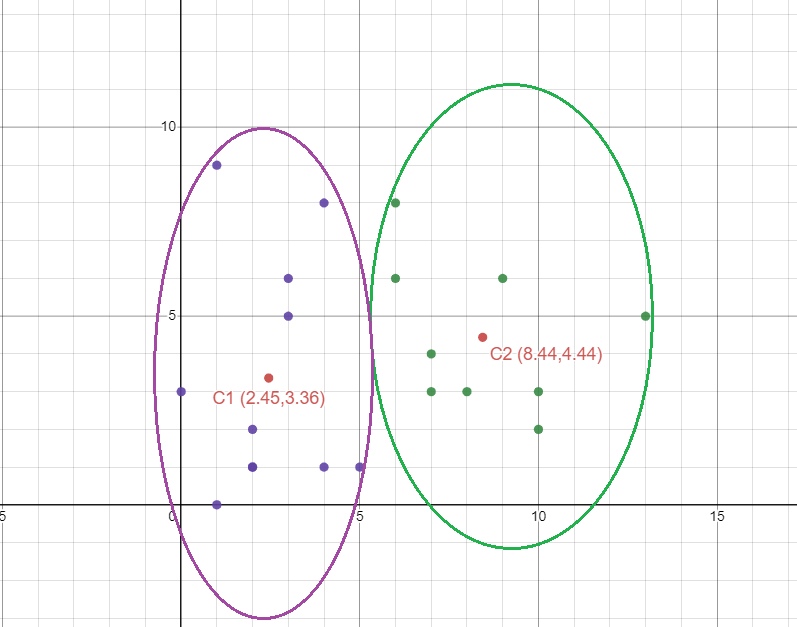
\includegraphics[width=14cm]{Clusters K = 2}
    \newline
    \textbf{K Means, K = 3}\par\medskip
    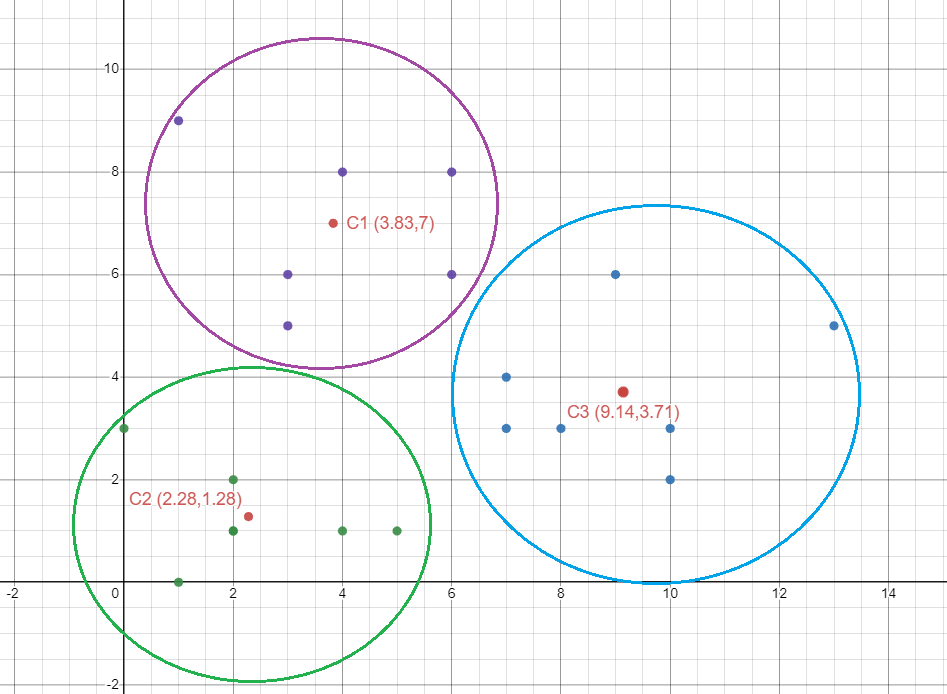
\includegraphics[width=15cm]{Clusters K = 3}
\end{figure}

\clearpage
\section*{Perceptron}
My perceptron algorithm using the data from "perceptron\textunderscore2.csv" ran until 3 epochs with the weight vector as [2.0, 4.0] and bias term as 2. It perfectly linearly separates the positive 1 labels and the negative -1 labels. I graphed the plot using matplotlib in Python. First, I plotted the points on the graph. Then I calculated the line. Since w1*x + w2*y + b = 0, the equation can be formed such that y = ((-w1*x)/w2) + (-b/w2). Plugging in the weight vector and bias, the equation comes out to y = (-2/4)*x + (-2/4) = -0.5x-0.5. The weight vector on the graph points towards the positive values while values in the opposite direction are negative. This means that anything above the green line is positive with label 1 and anything below the green line is negative with label -1.

\begin{figure}[!htb]
    \centering
    \textbf{Perceptron Output}\par\medskip
    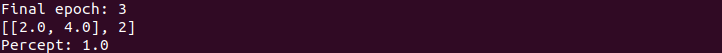
\includegraphics[width=15cm]{Project 2 Perceptron}
    \newline
    \newline
    \textbf{Perceptron Plot}\par\medskip
    \frame{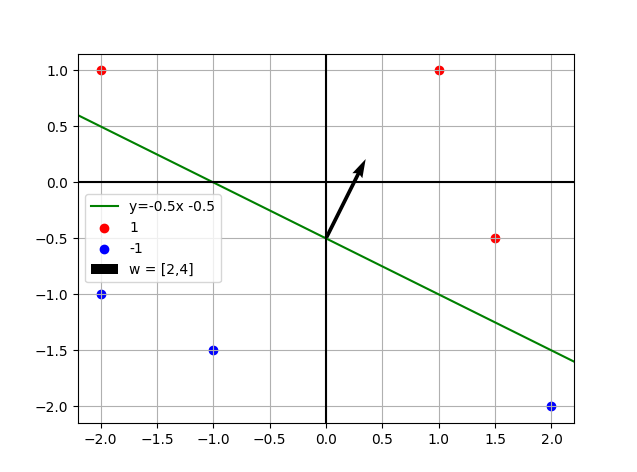
\includegraphics[width=15cm]{Project 2 Perceptron Plot}}
\end{figure}
\end{document}
